\chapter{Empirical priors: visceral leishmaniasis}
\label{applications-priors_empirical}

Another common patten in global data availability is exemplified by
the data gathered in the systematic review for Visceral Leishmaniasis
(VL).  For VL, there are a few regions for which detailed data on the
age pattern of disease incidence was available, but many more regions
where incident cases were reported without age-specificity.
Hierarchical modeling using an empirical Bayesian prior is our way to
conduct partial pooling, and borrow strength from the regions with
age-specific data to produce estimates of age patterns in regions
where little or no age-specific data is available.  This chapter shows
the application of empirical priors to estimating VL incidence in
sub-Saharan Africa by borrowing strength from Latin America.

VL is a parasitic disease in which the parasite
invades cells in the liver, spleen, bone marrow and lymph nodes.  If
untreated, it causes life-threatening systemic infection.  Diagnosis
includes identification of the parasite in tissue samples, ideally
from the spleen or bone marrow.  The parasite is transmitted by
several species of sandflies.  Traditionally endemic in the tropics,
subtropics and southern Europe, VL is becoming an AIDS-associated
opportunistic infection. \cite{herwaldt_leishmaniasis_1999,
baron_medical_1996}

Data are primarily from hospital admissions records, but also include
a handful of published studies.  Only population
representative data were included for the analysis, specific
subpopulation groups and cases of HIV-coinfection were excluded.  Thus
the analysis includes $3583$ data points from $12$ GBD 2010 study regions.

    \begin{figure}[h]
        \begin{center}
            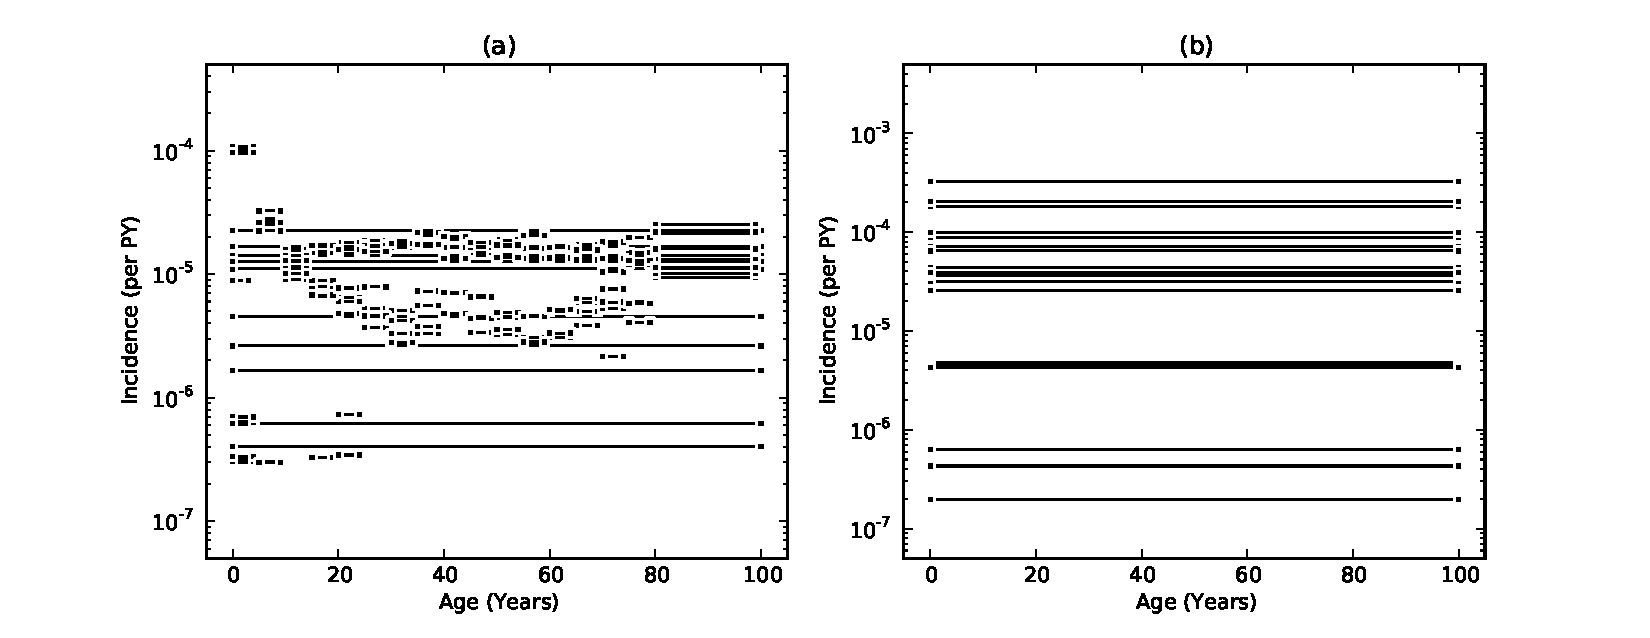
\includegraphics[width=\textwidth]{vl-data.pdf}
            \caption{Visceral leishmaniasis incidence data from
              systematic review for GBD 2010 study.  Data from Latin
              America and the Caribbean are shown in panel (a), and
              data sub-Saharan Africa are shown in panel (b).  The
              levels of the data are extremely heterogeneous; note
              that even displaying them requires a log-scale on the
              $y$-axis.}
            \label{fig:app-vl data}
        \end{center}
    \end{figure}

The data from the cluster of regions composed of the Caribbean,
central, Andean and tropical Latin America, has low incidence.
However it has an age-pattern that can be used as an empirical prior
for areas without an age-pattern, such as the regions in sub-Saharan
Africa.  Figure \ref{fig:app-vl data} shows the available data for
these clusters of regions.

Estimates using only data from sub-Saharan Africa would have no way to
estimate the age pattern of disease incidence. By borrowing strength
from the Latin America region cluster, it is possible to estimate an
age pattern for incidence in sub-Saharan African countries that is
informed by the levels observed in the non-age-specific data.  The
empirical bayes approach to this is shown in Figure \ref{fig:app-vl
  pred compare}.

    \begin{figure}[h]
        \begin{center}
            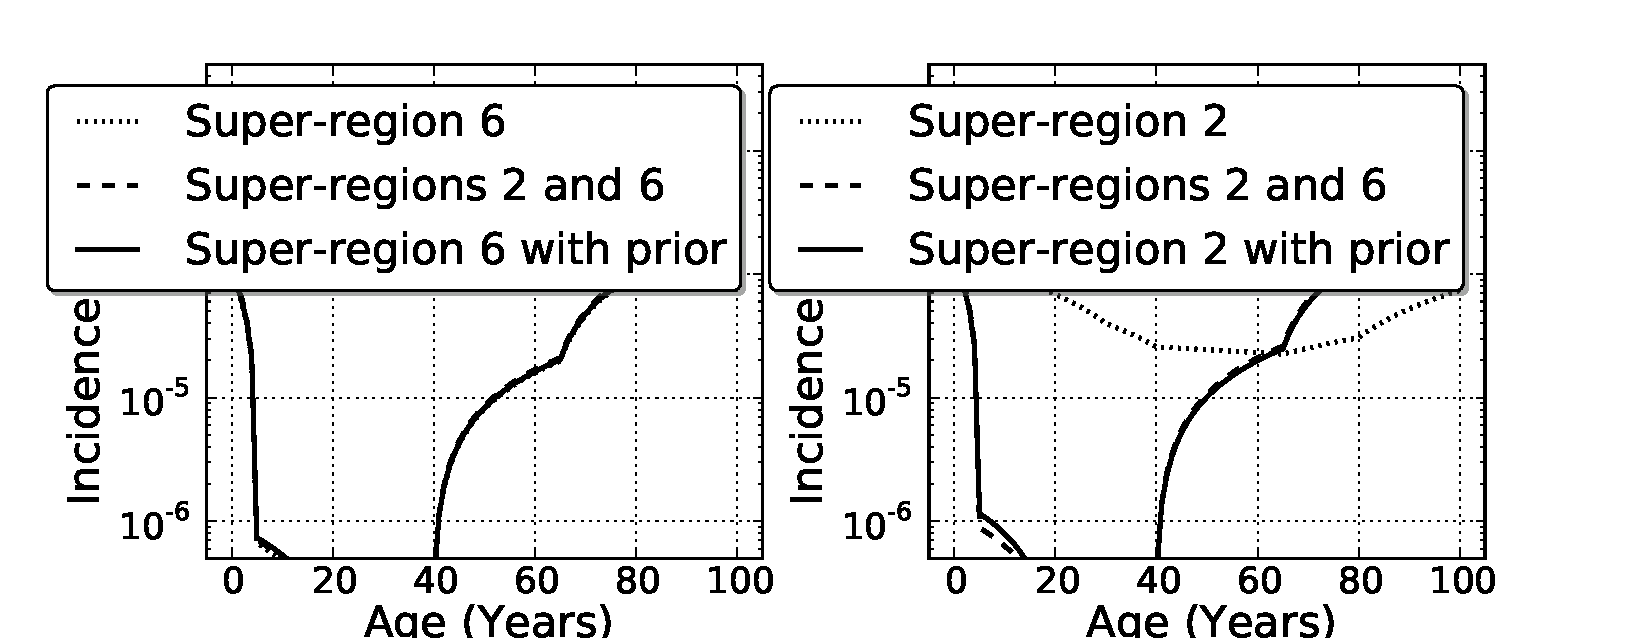
\includegraphics[width=\textwidth]{vl-pred_compare.pdf}
            \caption{A comparison of incidence estimates for males in
              super-region 6 (panel (a)) and super-region 2 (panel
              (b)) using data solely from that geographical area, data
              from both areas and data solely from that area with the
              estimate from both areas as an empirical prior.}
            \label{fig:app-vl pred compare}
        \end{center}
    \end{figure}
